% =========================================================
% DIAGRAMA: Arquitectura general del sistema
% Archivo imagen: Ilustraciones/arch_general.png
%
% QUÉ DIBUJAR EN DRAW.IO:
%   Vista de bloques con 3 nodos principales y las capas de protocolo entre ellos.
%
%   ┌──────────────────┐     CAN Bus 500kbps      ┌──────────────────────┐
%   │  Arduino MKR     │ ◄──────────────────────► │  Raspberry Pi        │
%   │  + CAN Shield    │    ISO 11898 (física)     │                      │
%   │                  │    ISO 15765-2 (ISO-TP)   │  Python 3            │
%   │  ECU Simulator   │    SAE J1979 (OBD-II)    │  ├─ IsoTpTransport   │
%   │  ├─ Mode 01/03   │                           │  ├─ DiagnosticSession│
%   │  ├─ Mode 04/09   │                           │  ├─ BleGattServer    │
%   │  ├─ ISO-TP SF/FF │                           │  └─ SqliteLogger     │
%   │  └─ CAN Noise    │                           │                      │
%   └──────────────────┘                           │  SQLite diagnostics.db│
%                                                  └──────────┬───────────┘
%                                                             │
%                                                    BLE 2.4 GHz
%                                                    GATT / NUS
%                                                    JSON over NUS
%                                                             │
%                                              ┌──────────────▼───────────┐
%                                              │  App Móvil               │
%                                              │  React Native + Expo     │
%                                              │  ├─ ConnectionScreen     │
%                                              │  ├─ DashboardScreen      │
%                                              │  ├─ DtcScreen            │
%                                              │  ├─ LogsScreen           │
%                                              │  └─ ConsoleScreen        │
%                                              │  Zustand state stores    │
%                                              └──────────────────────────┘
%
%   Detalles adicionales a mostrar:
%   - Junto al bus CAN: flecha bidireccional con etiquetas:
%       TX: 0x7E0 | RX: 0x7E8 | 500 kbps
%   - Junto al BLE: flecha bidireccional con:
%       NUS UUID: 6E400001-... | MTU: 240 bytes
%   - En el Arduino: botón D7 (ignición) y botón D6 (DTC fault) como componentes externos
%   - En la Raspberry Pi: icono cilindro para SQLite
%   - Leyenda de colores por capa de protocolo:
%       Rojo = Capa física (CAN/BLE radio)
%       Naranja = Capa transporte (ISO-TP / ATT)
%       Verde = Capa aplicación (OBD-II / NUS JSON)
%   - Título: "Arquitectura general del sistema de monitorización OBD-II"
% =========================================================

\begin{figure}[!htbp]
\centering
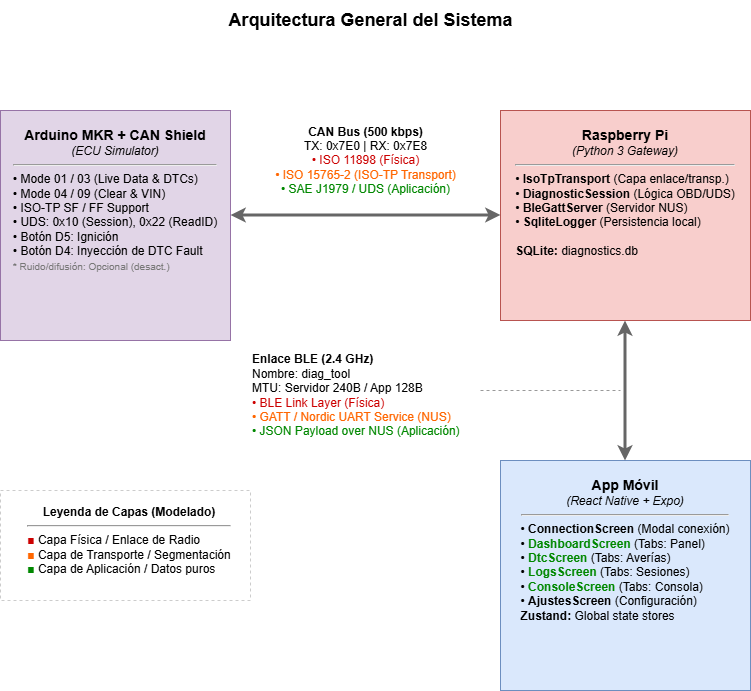
\includegraphics[width=\textwidth]{Ilustraciones/arch_general.png}
\caption{Arquitectura general del sistema. El simulador Arduino genera tráfico OBD-II y ruido CAN sobre bus CAN a 500~kbps. La Raspberry Pi actúa como escáner ISO-TP, decodifica las respuestas, las persiste en SQLite y las expone vía BLE GATT (servicio NUS). La aplicación móvil React Native se conecta por BLE y presenta los datos en tiempo real.}
\label{fig:arch_general}
\end{figure}
